\chapter{Considerações Gerais}
\label{cap:02}

\section{Engenharia de Software e Qualidade}

A Engenharia de Software compreende a aplicação de abordagens sistemáticas, disciplinadas e quantificáveis ao desenvolvimento, à operação e à manutenção de sistemas \cite{Valente2020}. Como a computação está presente em grande parte das atividades contemporâneas, assegurar a confiabilidade e a estabilidade das aplicações tornou-se uma exigência fundamental, e não apenas um diferencial técnico.

Embora os níveis de complexidade e os riscos envolvidos variem conforme o domínio, a aplicação de princípios de engenharia permanece indispensável. Essa necessidade é evidenciada em sistemas de segurança crítica, nos quais falhas de software podem resultar em consequências catastróficas. Um exemplo histórico notável é o caso do acelerador linear Therac-25, cujas falhas de software e de projeto contribuíram para acidentes de superexposição à radiação, alguns deles fatais \cite{turner1993investigation}.

A relevância da qualidade, porém, não se restringe a cenários de alto risco. Mesmo que um sistema de gestão de uma padaria não tenha a mesma complexidade ou criticidade de um sistema bancário, médico ou militar, ambos precisam ser confiáveis e sustentáveis ao longo do tempo. Em qualquer escala, o software deve preservar a experiência do usuário e a integridade dos processos que apoia.

A manutenção de padrões de qualidade em projetos colaborativos, portanto, torna-se um desafio crescente. À medida que um sistema evolui, a complexidade técnica e a densidade do código também aumentam, tornando processos de verificação exclusivamente manuais pouco viáveis e sujeitos a falhas humanas.

\section{Teste de Software}

O teste de software busca, por meio de um conjunto finito de casos, verificar e validar (V\&V) se a aplicação atende aos requisitos esperados \cite{Valente2020}. Essa etapa representa um investimento significativo e pode consumir parcela expressiva do tempo e do custo total do desenvolvimento de um sistema \cite{Myers2014}.

Esse processo inicia-se em componentes individuais ou pequenos módulos, com o objetivo de identificar falhas lógicas e de dados. Após essa validação inicial, os componentes são integrados ao sistema para testes de ordem superior, cujo objetivo é assegurar que o software atenda aos requisitos do cliente \cite{Sommerville2019}. \cite{Myers2014} destaca que o teste não deve ser entendido apenas como uma forma de demonstrar que o software funciona, mas como um processo orientado à busca de falhas. Nessa perspectiva, um teste pode ser considerado bem-sucedido quando revela um erro ainda não descoberto. Em sistemas cada vez mais complexos, aplicar essa abordagem apenas de forma manual torna-se exaustivo e sujeito a vieses, reforçando a necessidade de apoio automatizado.

\subsection{Teste Estrutural (Caixa Branca)}

O teste estrutural, também conhecido como teste de caixa branca, concentra-se na análise da lógica interna do programa \cite{Delamaro2013}. Ao contrário do teste de caixa preta, que observa se entradas e saídas correspondem ao esperado, essa técnica exige acesso ao código-fonte para avaliar caminhos de execução, \textit{loops} e condições lógicas.

Sua relevância reside na capacidade de orientar a verificação das estruturas internas do programa. Isso inclui apoiar a identificação de instruções, desvios lógicos (verdadeiro e falso), laços de repetição e caminhos independentes que devem ser considerados durante o planejamento dos testes.

\subsubsection{Grafo de Fluxo de Controle (GFC)}

O Grafo de Fluxo de Controle (GFC) é uma representação gráfica usada na análise estrutural. Ele modela a lógica do programa como um grafo dirigido, em que os \textbf{nós} representam blocos de processamento sequencial, sem desvios, e as \textbf{arestas} representam o fluxo de controle entre esses nós.

Entre os elementos do GFC estão os nós de predicado, que correspondem a pontos de decisão no código, como \texttt{if} ou \texttt{while}, dos quais partem múltiplas arestas. Ferramentas de teste e análise estática utilizam o GFC para calcular caminhos independentes e determinar a complexidade lógica do algoritmo, transformando o código textual em uma estrutura matemática navegável.

\pagebreak

Para consolidar o entendimento sobre a relação entre o código-fonte, o Grafo de Fluxo de Controle (GFC) e a Complexidade Ciclomática, apresenta-se a seguir um algoritmo simples de verificação condicional.

\lstinputlisting[language=Python, caption={Algoritmo de verificação condicional.}, numbers=left]{fontes/codigos/exemplo-status.py}
\label{lst:verifica_status}

A partir da análise do Código \ref{lst:verifica_status}, é possível mapear a lógica para uma representação visual. A Figura \ref{fig:exemplo_gfc} ilustra o GFC correspondente, na qual os blocos de comando se tornam nós e o fluxo de execução é representado por arestas direcionadas.

\begin{figure}[H]
    \centering
      \caption{Exemplo de GFC.}
    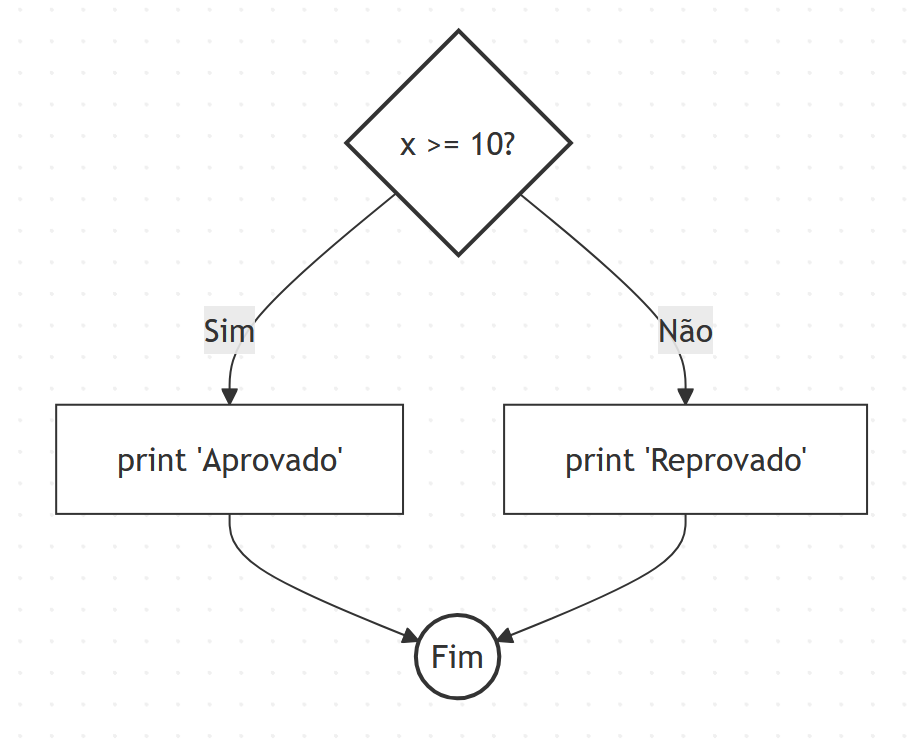
\includegraphics[width=0.5\linewidth]{fontes/imagens/diagramas/exemplo-gfc.png}

    \label{fig:exemplo_gfc}
    \fonte{Elaborada pelo autor.}
\end{figure}

\subsubsection{Complexidade Ciclomática - V(G)}

A Complexidade Ciclomática é uma métrica de software desenvolvida por Thomas McCabe em 1976. Ela quantifica a complexidade lógica de um programa a partir do número de caminhos linearmente independentes em seu Grafo de Fluxo de Controle \cite{McCabe1976}.

A métrica é calculada pela fórmula $V(G) = E - N + 2P$, em que $E$ é o número de arestas, $N$ é o número de nós e $P$ é o número de componentes conexos do grafo. Em grafos com apenas um componente conexo, essa expressão simplifica-se para $V(G) = E - N + 2$. No modelo de teste de caminhos básicos, o valor de $V(G)$ corresponde à dimensão de uma base de caminhos linearmente independentes do GFC. Isso não representa todos os caminhos possíveis de execução, sobretudo quando há laços, nem garante a detecção de todos os defeitos. A equivalência $V(G)=d+1$, em que $d$ é o número de decisões, depende de um grafo conectado e da forma como predicados e condições compostas são modelados; expressões com curto-circuito, como \texttt{and} e \texttt{or}, podem alterar essa contagem. McCabe propõe o valor 10 como uma referência para sinalizar módulos que merecem revisão, e não como um limite universal de qualidade \cite{McCabe1976}.

\subsection{Cálculo da Complexidade Ciclomática}
Com base na representação visual da Figura \ref{fig:exemplo_gfc}, é possível aplicar a métrica de McCabe para determinar a complexidade lógica $V(G)$. Observando o grafo, identificam-se os seguintes elementos:

\begin{itemize}
    \item \textbf{Nós ($N$):} 4 (Início/If, Print Aprovado, Print Reprovado, Fim).
    \item \textbf{Arestas ($E$):} 4 (As conexões entre os nós).
    \item \textbf{Componentes conexos ($P$):} 1 (há um único componente conexo).
\end{itemize}

Aplicando a fórmula fundamental de McCabe:

\begin{equation}
    V(G) = E - N + 2P
\end{equation}

Substituindo pelos valores extraídos do grafo:

\[
    V(G) = 4 - 4 + 2(1) = 2
\]

O resultado $V(G) = 2$ indica que uma base do GFC pode conter dois caminhos linearmente independentes: (1) o caminho em que a condição é verdadeira e (2) o caminho em que ela é falsa. No teste de caminhos básicos, esses caminhos orientam a seleção de casos de teste para exercitar os dois ramos da função. A quantidade não é um limite universal para todos os caminhos de execução nem assegura a ausência de falhas. Ela também não deve ser confundida com a quantidade de caminhos que um algoritmo enumera: essa lista concreta depende do critério de modelagem e do procedimento de geração. A validação dos caminhos produzidos pelo GUY deve, portanto, verificar explicitamente sua independência, conforme o protocolo da Seção \ref{sec:validacao_guy}.



\section{Análise Estática de Código}

A análise estática de código consiste no exame do software sem executá-lo. Essa técnica é adequada para a inspeção estrutural, pois permite verificar a base de código em busca de padrões sintáticos, violações de regras e métricas de complexidade ainda durante o desenvolvimento.

Diferencia-se da análise dinâmica, que requer a execução do programa com dados de teste reais para observar comportamentos em tempo de execução (como uso de memória e falhas). Aplicações práticas da análise estática incluem a detecção precoce de defeitos, a verificação de conformidade com guias de estilo e o cálculo automático de métricas como a complexidade ciclomática, fornecendo retorno ao desenvolvedor durante o desenvolvimento.

\subsection{Processamento Léxico e Sintático}

Para construir o GFC e realizar a análise estática, o GUY utiliza conceitos de compiladores. O processo inicia-se com a \textbf{tokenização} (análise léxica), que divide o código-fonte em unidades mínimas de significado (tokens) \cite{Cooper2012}.

Em seguida, realiza-se a identificação de estruturas através da \textbf{análise sintática}, que organiza esses \textit{tokens} em uma Árvore Sintática Abstrata (AST). A AST é uma representação hierárquica que expõe a estrutura gramatical do código \cite{Aho1995}. Ao percorrer a AST, a ferramenta identifica onde começam e terminam os blocos lógicos (funções, laços e condicionais) para, a partir disso, desenhar os nós e arestas do GFC e calcular a complexidade.

\section{Tecnologias e Linguagens Adotadas}

O GUY adota uma arquitetura de extensão para o \textit{Visual Studio Code} (VS Code) \cite{microsoft_vscode}. A lógica principal executa no \textit{Extension Host}, utilizando Node.js e TypeScript para acessar o arquivo aberto no editor, acionar a análise estática e coordenar a comunicação com a interface. Na camada visual, a biblioteca React é utilizada em uma \textit{Webview}. A visualização do GFC é implementada com \texttt{@xyflow/react}, e o posicionamento dos nós é apoiado por \texttt{@dagrejs/dagre} \cite{react_docs,xyflowReactWeb,dagreWeb}.

Para o processamento de código e a análise sintática (\textit{parsing}), a implementação utiliza o \textbf{Tree-sitter} com a gramática de Python \cite{TreeSitterWeb}. O resultado é percorrido para identificar as estruturas necessárias à construção do GFC. O ANTLR é uma alternativa de geração de analisadores considerada na fundamentação, mas não integra a implementação descrita neste trabalho \cite{ANTLRWeb}.

A troca da gramática, por si só, não fornece suporte a uma nova linguagem: cada linguagem exige um mapeamento próprio de seus nós sintáticos para o modelo de GFC e a validação correspondente. No núcleo de visualização, Cytoscape.js e D3.js são alternativas possíveis, mas não são bibliotecas adotadas pela implementação atual \cite{CytoscapeWeb,D3Web}.


\section{Trabalhos Correlatos}

A pesquisa bibliográfica identificou ferramentas e algoritmos que exploram a representação gráfica de programas para apoiar a compreensão e o teste de software. A seguir, são descritas três abordagens: um algoritmo de layout focado na legibilidade de fluxo (VEIL), uma ferramenta de documentação (Code2Flow) e uma solução de análise estática (CodeSurfer).

\subsection{VEIL (\textit{Vertical Execution-order Informed Layout})}
O VEIL é um algoritmo de desenho de grafos descrito por \cite{veil}, desenvolvido para alinhar a visualização de Grafos de Fluxo de Controle (GFC) à leitura de código-fonte. A abordagem utiliza análise de dominadores e propõe critérios de organização visual, entre eles o \textit{Happens-Before} (C10) e o \textit{Edge Direction Grouping} (C11) \cite{veil}.

A principal distinção está no escopo. O VEIL trata da organização visual do grafo. O GUY utiliza a visualização do GFC para apresentar a Complexidade Ciclomática e os caminhos associados no ambiente de desenvolvimento; a efetividade desse uso educacional não é avaliada nesta fundamentação.

\subsection{CodeSurfer}
O CodeSurfer, desenvolvido pela GrammaTech, é uma ferramenta de análise estática e navegação em código-fonte (C/C++) \cite{codesurfer}. Ao contrário de IDEs comuns, sua documentação descreve a construção de informações de dependência que permitem navegar pelo Grafo de Fluxo de Controle e pelo Grafo de Dependência de Dados de funções.

A distinção em relação ao trabalho proposto está no público-alvo e no escopo. O CodeSurfer é descrito como uma ferramenta para análise e manutenção de software. A ferramenta aqui desenvolvida gera GFCs no ambiente local do VS Code e apresenta a métrica no contexto definido pelo projeto; não se afirma, com base apenas nessa comparação, redução de barreiras de entrada ou equivalência funcional.

\subsection{Code2Flow}
O Code2Flow é uma ferramenta que converte pseudocódigo e código em fluxogramas interativos, conforme sua documentação \cite{code2flow}. Seu uso descrito concentra-se na documentação de processos e na comunicação da lógica entre participantes, a partir de texto.

O Code2Flow foca na representação de processos de negócio e lógica geral. Essa finalidade pode abstrair detalhes técnicos necessários ao teste estrutural. Em comparação com o escopo descrito para o GUY, sua documentação não apresenta cálculo explícito da Complexidade Ciclomática nem critérios de cobertura de teste.
